% atsresume-doc.tex: documentation for the atsresume class.
% Compile with pdflatex after atsresume-example.tex, whose PDF is shown
% on the first page.
%
% Copyright (C) 2026 Super Lede. Part of the atsresume work, distributed
% under the LaTeX Project Public License 1.3c or later.
\documentclass[11pt]{article}
\usepackage[T1]{fontenc}
\usepackage{tgpagella}
\renewcommand\ttdefault{lmtt}
\usepackage[margin=1in]{geometry}
\usepackage{graphicx}
\usepackage{fancyvrb}
\usepackage[hidelinks]{hyperref}
\hypersetup{pdftitle={The atsresume class}, pdfauthor={Super Lede}}

\fvset{xleftmargin=1em, fontsize=\small}
\newcommand\cs[1]{\texttt{\textbackslash#1}}
\newcommand\param[1]{\textrm{\textit{#1}}}
\setlength\parindent{0pt}
\setlength\parskip{0.6\baselineskip}
\raggedright

\title{The \texttt{atsresume} class}
\author{Super Lede\\\small templates@readableresume.com}
\date{Version 1.0.0, 2026-10-20}

\begin{document}
\maketitle

\section{What it's for}

Many employers run resumes through an applicant tracking system (ATS). The
system takes the text out of your PDF and sorts it into fields: name, email,
each job with its dates, each school. If the text comes out in the wrong
order, with words broken in two or letters swapped for odd characters, the
fields can come out wrong or empty, and a recruiter searching for a skill
you have might not find your resume.

\texttt{atsresume} is a class for a one-page resume that keeps its text in
reading order, with ligatures and hyphenation turned off. The layout is the Classic template from ReadableResume
(\url{https://readableresume.com}), where the same design is available for
Google Docs and Word: a single column, your name centered at the top,
section headings in capitals over a thin rule, and places and dates on the
right margin. Figure~\ref{fig:example} shows the example that comes with the
class.

\begin{figure}[ht]
  \centering
  \fbox{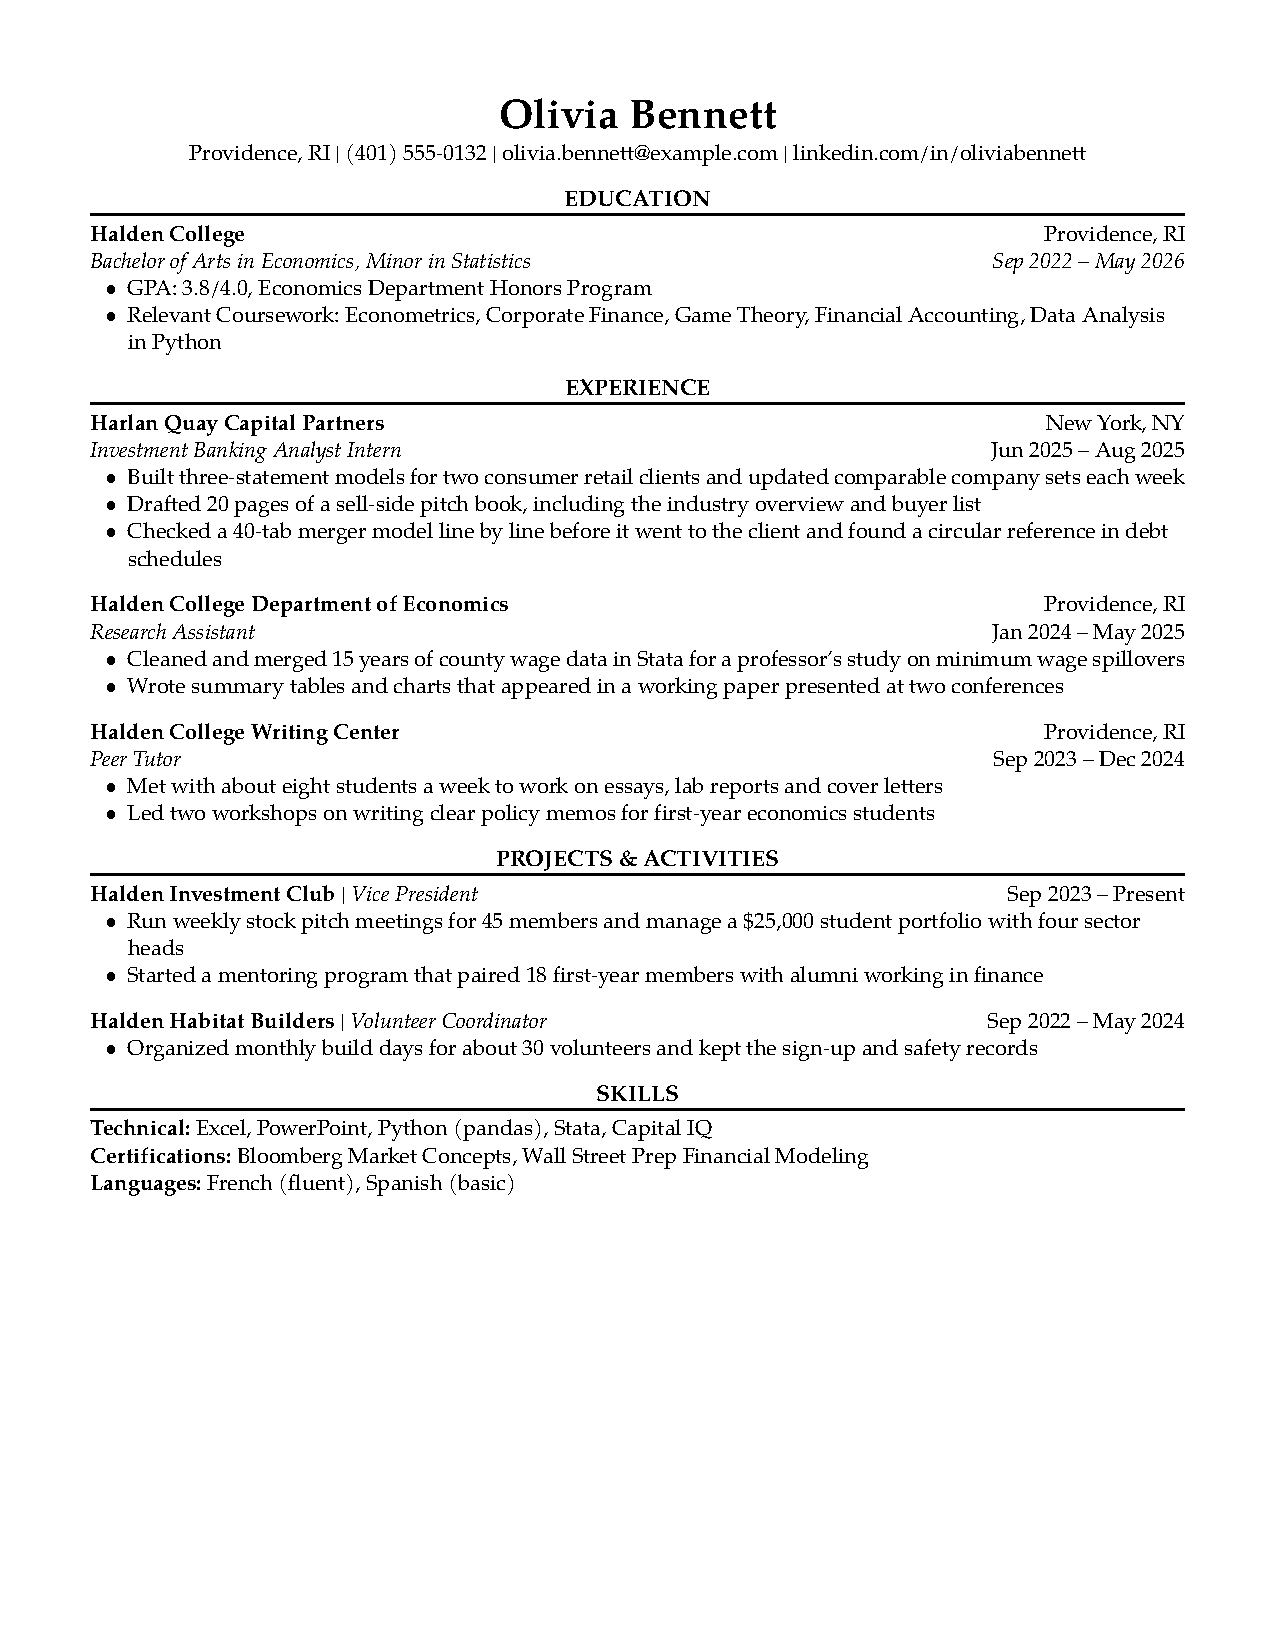
\includegraphics[width=0.62\linewidth]{atsresume-example.pdf}}
  \caption{\texttt{atsresume-example.tex}, compiled on US Letter paper.}
  \label{fig:example}
\end{figure}

\section{Getting started}

Copy \texttt{atsresume-example.tex}, replace the details with yours and
compile it with \texttt{pdflatex}, \texttt{lualatex} or \texttt{xelatex}.
Or start from this:

\begin{Verbatim}
\documentclass{atsresume}
\name{Your Name}
\contact{City, ST}
\contact{(555) 555-0100}
\contact{\email{you@example.com}}
\contact{\weblink{linkedin.com/in/yourname}}

\begin{document}
\makeheader

\section{Experience}
\experience{Company}{City, ST}{Job Title}{Jun 2024 – Present}
\begin{itemize}
  \item What you did, with a number if you have one
\end{itemize}

\section{Education}
\education{University}{City, ST}{Bachelor of Science in Biology}{May 2024}

\section{Skills}
\skill{Technical}{Excel, SQL, Python}
\skill{Languages}{Spanish (fluent)}
\end{document}
\end{Verbatim}

The class reads UTF-8, so you can type an en dash in a date range as
\texttt{–} or as \texttt{-{}-}.

\section{Commands}

\subsection*{The header}

\begin{description}
\item[\cs{name}\{\param{Your Name}\}] Your name, centered at the top. Put it in
  the preamble. It also becomes the PDF's author and, followed by
  ``Resume'', its title.
\item[\cs{contact}\{\param{item}\}] One item of the contact line. Use it once
  per item, in the order you want them; they're joined with vertical bars.
  An item never breaks across two lines; if the line is too long it wraps
  between items.
\item[\cs{email}\{\param{address}\}] An email address, as a link. Type it
  as it is: characters such as \verb|_| need no backslash, and one typed out
  of habit is dropped, so \verb|first\_last@example.com| and
  \verb|first_last@example.com| give the same address. The one exception
  is \verb|%|, which has to be typed \verb|\%| because TeX reads a bare
  \verb|%| as the start of a comment. The same goes for \cs{weblink}.
\item[\cs{weblink}\{\param{address}\}] A web address, as a link. It's shown
  as you type it. If you leave out \texttt{https://}, the link gets it
  anyway, so \verb|\weblink{linkedin.com/in/you}| shows the short form and
  still opens the page.
\item[\cs{makeheader}] Prints the name and the contact line. Put it right
  after \verb|\begin{document}|.
\end{description}

\subsection*{Sections}

\begin{description}
\item[\cs{section}\{\param{Title}\}] A section heading, centered, in capitals,
  over a rule. Type the title in any case. Sections aren't numbered, and
  \cs{section*} does the same thing.
\end{description}

\subsection*{Entries}

Each entry command prints the lines of one job, school or activity. A list
of bullet points, in an ordinary \texttt{itemize} environment, can follow
it. Leave an argument empty to skip it: \verb|\experience{Company}{}{Job Title}{}|
prints no place and no dates.

\begin{description}
\item[\cs{education}\{\param{School}\}\{\param{Place}\}\{\param{Degree}\}\{\param{Dates}\}]
  The school in bold with the place on the right, then the degree and the
  dates in italics.
\item[\cs{experience}\{\param{Company}\}\{\param{Place}\}\{\param{Job title}\}\{\param{Dates}\}]
  The company in bold with the place on the right, then the job title in
  italics with the dates on the right.
\item[\cs{activity}\{\param{Name}\}\{\param{Role}\}\{\param{Dates}\}]
  One line: the name in bold, a vertical bar, the role in italics, and the
  dates on the right. Use it for clubs, volunteering, projects or
  certifications.
\item[\cs{skill}\{\param{Label}\}\{\param{Text}\}]
  One line with a bold label, such as \verb|\skill{Languages}{French (fluent)}|.
\end{description}

When the left part of a line is too long for the place or the dates to fit
beside it, they move to the next line, still on the right margin.

Plain paragraphs work anywhere, for example a short summary under a
\cs{section}\verb|{Summary}|.

\section{Paper size}

The default is US Letter with 0.6\,in margins. For A4 with 15\,mm margins,
use \verb|\documentclass[a4paper]{atsresume}|. These are the margins of the
original template. To change them, use \cs{geometry} in the preamble, for
example \verb|\geometry{margin=0.75in}|.

The text is 10.5\,pt, the name 20\,pt and the section headings 11\,pt, the
sizes of the original. The \texttt{10pt}, \texttt{11pt} and \texttt{12pt}
options of the standard classes have no effect.

\section{Fonts}

The text is set in TeX Gyre Pagella: the Type~1 version with pdfLaTeX, the
OpenType version with LuaLaTeX and XeLaTeX, so the page looks the same with
each engine. Pagella is part of TeX Live, and on Debian and Ubuntu it comes
in the \texttt{tex-gyre} and \texttt{fonts-texgyre} packages. Its letters
are about as wide as those of Georgia, the font of the original template, so
lines break in nearly the same places.

To use another font, load it after the class. With pdfLaTeX, load its
package:
\begin{Verbatim}
\documentclass{atsresume}
\usepackage{gelasio}
\end{Verbatim}
With LuaLaTeX or XeLaTeX, use \cs{setmainfont} and keep
\verb|Ligatures={TeX,NoCommon}|, which turns off the ligatures for the new
font too (see the next section):
\begin{Verbatim}
\setmainfont{Gelasio}[Extension=.otf, UprightFont=*-Regular,
  BoldFont=*-Bold, ItalicFont=*-Italic, BoldItalicFont=*-BoldItalic,
  Ligatures={TeX,NoCommon}]
\end{Verbatim}
Gelasio, a free font drawn to the same measurements as Georgia, is in TeX
Live's full installation.

\section{What the class does for parsers}

\begin{itemize}
\item \textbf{One column, stored in reading order.} Places and dates are
  pushed to the right margin with glue on the same line as the company or
  title, not set in a table, a second column or a box at a fixed position.
  The PDF stores each line left to right, top to bottom, so a parser reads
  ``Halden College Providence, RI'' rather than a column of places after a
  column of names.
\item \textbf{No ligatures.} Fonts normally join letters such as f and i
  into one glyph. Some readers turn that glyph into a single character
  (Unicode U+FB01) that doesn't match ``fi'' when an ATS searches for
  ``finance''. The class turns these ligatures off; \verb|--| and
  \verb|``| still give an en dash and a quotation mark.
\item \textbf{No hyphenation.} A word split across two lines can reach a
  parser as two fragments, so hyphenation is off.
\item \textbf{Real characters.} Bullets are the text font's bullet,
  Unicode U+2022, which parsers recognize. With pdfLaTeX every glyph also
  gets a Unicode mapping (\cs{pdfgentounicode}), so copied text matches what
  you typed.
\item \textbf{Page breaks.} A section heading, or the first lines of an
  entry, never sit alone at the bottom of a page, and a bullet point never
  splits across two pages.
\item \textbf{Links and metadata.} Email and web addresses are links, and
  the PDF's title and author are set from \cs{name}.
\end{itemize}

What the class can't stop is text added outside these commands: icons
instead of words, two \texttt{minipage}s side by side, text in a table or
in a picture. Many parsers have trouble with them. If you add any, check
the extracted text as described in the next section.

\section{Checking your PDF}

Open the PDF, select all the text, copy it and paste it into a plain text
editor. You should get every word, in the order you read the page, with
each place and date right after the line it belongs to.

On the command line, poppler's \texttt{pdftotext} does the same:
\begin{Verbatim}
pdftotext -layout resume.pdf -
\end{Verbatim}
Without \texttt{-layout}, pdftotext tries to find columns on the page. When
an entry's bullet points are short, it can take the place and dates for a
column of their own and print them after that entry's bullets. The PDF
still stores them in order, and pdftotext does the same with right-aligned
dates from a word processor.

The example that comes with the class was compiled with pdfLaTeX, LuaLaTeX
and XeLaTeX, on US Letter and on A4. In each of the six PDFs,
\texttt{pdftotext -layout} gave back the text word for word and in reading
order, and OpenResume, an open-source resume parser, returned every value it
reads exactly as written: the name and contact details, each job, school and
project with its dates, and every bullet point and skills line. How well a
particular ATS fills in its own fields still depends on that system.

\section{License}

Copyright 2026 Super Lede. This work may be distributed and/or modified
under the conditions of the LaTeX Project Public License, version 1.3c or
later. It has the LPPL maintenance status ``maintained''; the current
maintainer is Super Lede. The work consists of \texttt{atsresume.cls},
\texttt{atsresume-example.tex} and \texttt{atsresume-doc.tex}.

The person, schools and companies in the example are made up.

Questions and bug reports are welcome at templates@readableresume.com.

\end{document}
